\section{Exploration et préparation des données}

\subsection{Collecte, intégration, nettoyage et prétraitement}

La collecte s'est appuyée sur \textbf{ScrapeGraphAI}, un service d'extraction piloté par IA auquel on soumet une URL,
un schéma JSON cible et une consigne en langage naturel, plutôt que des sélecteurs CSS statiques : ce choix
limite la maintenance face aux évolutions de structure des pages sources, au prix d'une variabilité que le
nettoyage a dû absorber en aval.

Deux sources hétérogènes ont été intégrées séparément plutôt que forcées dans un schéma commun.
\textbf{Clutch.co} fournit des taux horaires exprimés en dollars et des profils mobile/web distincts pour une
même entreprise ; \textbf{La Fabrique du Net} fournit des fourchettes de budget par projet en euros, une
tranche de taille de projet la plus courante, et l'intégralité des avis clients. Plutôt que de fusionner ces
deux structures dans une table de prix unique --- ce qui aurait exigé une conversion de devise et une perte
d'information sur des champs propres à chaque source (\texttt{tranche\_plus\_courante},
\texttt{evaluation\_tarifs} côté La Fabrique du Net ; \texttt{taux\_horaire} côté Clutch) --- le schéma
retient deux tables \texttt{etat\_marche} séparées, reliées à une table \texttt{competitors} commune ne
portant que l'identité (nom, URL, ville, \texttt{service\_type}).

Le nettoyage et le prétraitement ont porté sur trois points principaux :

\begin{itemize}
    \item \textbf{Dédoublonnage à clé composite.} L'unicité d'une entreprise n'est pas définie par son URL
    seule mais par le couple \texttt{(url\_profil, service\_type)} : une même agence peut avoir un profil
    Clutch mobile et un profil Clutch web distincts, avec des tarifs différents, qu'il aurait été incorrect
    de fusionner en une seule ligne.
    \item \textbf{Parsing des tarifs textuels en valeurs numériques.} Les taux horaires Clutch sont extraits
    sous forme de texte libre (\texttt{"\$50 - \$99 / hr"}, \texttt{"< \$25 /hr"}, \texttt{"\$150+ / hr"}).
    La fonction \texttt{parseTauxHoraire} normalise ces formats en un couple \texttt{(min, max)} numérique
    exploitable pour l'analyse statistique, en gérant explicitement les cas de borne ouverte (\texttt{<},
    \texttt{+}).
    \item \textbf{Traitement des valeurs manquantes et incohérentes.} Les champs renvoyés comme la chaîne
    littérale \texttt{"No content available"} par l'extracteur sont explicitement remis à \texttt{null}
    plutôt que conservés comme du texte, pour ne pas polluer les statistiques descriptives ou l'indexation
    vectorielle en aval.
    \item \textbf{Filtrage qualité des concurrents non exploitables.} Sur les 78 entreprises initialement
    identifiées et scrapées, certaines présentaient des champs clés systématiquement non renseignés par la
    source elle-même (\textit{"Min project size: Undisclosed"}, \textit{"Hourly rate: Undisclosed"}) et
    n'avaient par ailleurs aucun avis client associé. En l'absence de toute donnée exploitable, ni pour la
    couche tarifaire ni pour la couche sentiment, ces fiches ne pouvaient contribuer ni à l'analyse ni au
    système de recherche : elles ont donc été explicitement exclues plutôt que conservées avec des valeurs
    vides. C'est ce filtrage qui explique l'écart entre les 78 entreprises identifiées lors de la collecte et
    les 69 effectivement présentes dans la table \texttt{etat\_marche}.
\end{itemize}

Deux tables distinctes portent l'information issue des avis clients, et il est important de ne pas les
confondre. La table \texttt{etat\_marche} contient un champ \texttt{nombre\_avis}, qui correspond au nombre
d'avis brut tel qu'affiché par la source au moment du scraping ; ce chiffre n'est qu'indicatif et n'est pas
utilisé pour l'analyse de sentiment. Le chiffre qui fait réellement foi est le champ
\texttt{nb\_avis\_analyses} de la table \texttt{avis\_analyse}, qui correspond au nombre d'avis effectivement
traités par le module d'analyse de sentiment pour produire le \texttt{sentiment\_global}, le
\texttt{score\_sentiment} ainsi que les \texttt{points\_forts} et \texttt{points\_faibles} par concurrent. Ces
avis analysés proviennent de deux modes de collecte complémentaires : une partie a été récupérée par
scraping automatisé, l'autre a été collectée manuellement lorsque la source ne s'y prêtait pas ; les deux
sont fusionnés en amont de l'analyse de sentiment, sans distinction de traitement une fois intégrés à
\texttt{avis\_analyse}. Il en résulte qu'une entreprise peut afficher \texttt{note = 0} et
\texttt{nombre\_avis = 0} dans \texttt{etat\_marche} tout en disposant d'un \texttt{nb\_avis\_analyses} > 0
dans \texttt{avis\_analyse} : cela signifie que ses avis ont été collectés hors de Clutch/La Fabrique du
Net (autre plateforme, collecte manuelle), et non que l'entreprise est dépourvue de tout avis. Cette
distinction, exploitée en section 10.2 pour l'étude de corrélation note/sentiment, doit être gardée à
l'esprit dès l'intégration des données.

Le monitoring a été conçu comme un processus différentiel plutôt qu'un simple re-scraping périodique :
chaque relevé est comparé à l'état courant en base (\texttt{etat\_marche} /
\texttt{etat\_marche\_la\-fabri\-quedunet})
sur les seuls champs pertinents pour le prix, et une nouvelle ligne n'est insérée dans l'historique
append-only (\texttt{historique\_prix}) que si un changement réel est détecté. Ce choix limite le volume de
données stockées à du signal utile pour l'apprentissage de tendances futures, plutôt qu'à une accumulation de
mesures identiques. Chaque changement de prix ou de sentiment invalide par ailleurs l'embedding vectoriel
associé (mis à \texttt{null}), forçant son recalcul au prochain passage du pipeline d'indexation --- un
mécanisme de cohérence entre les données structurées et leur représentation vectorielle dans le RAG.

\subsection{Modèle relationnel des données}

Le schéma relationnel retenu sépare l'identité des concurrents, les deux formats de prix et l'analyse des avis, tout en les reliant par la clé \texttt{competitor\_id}.

\begin{figure}[H]
\centering
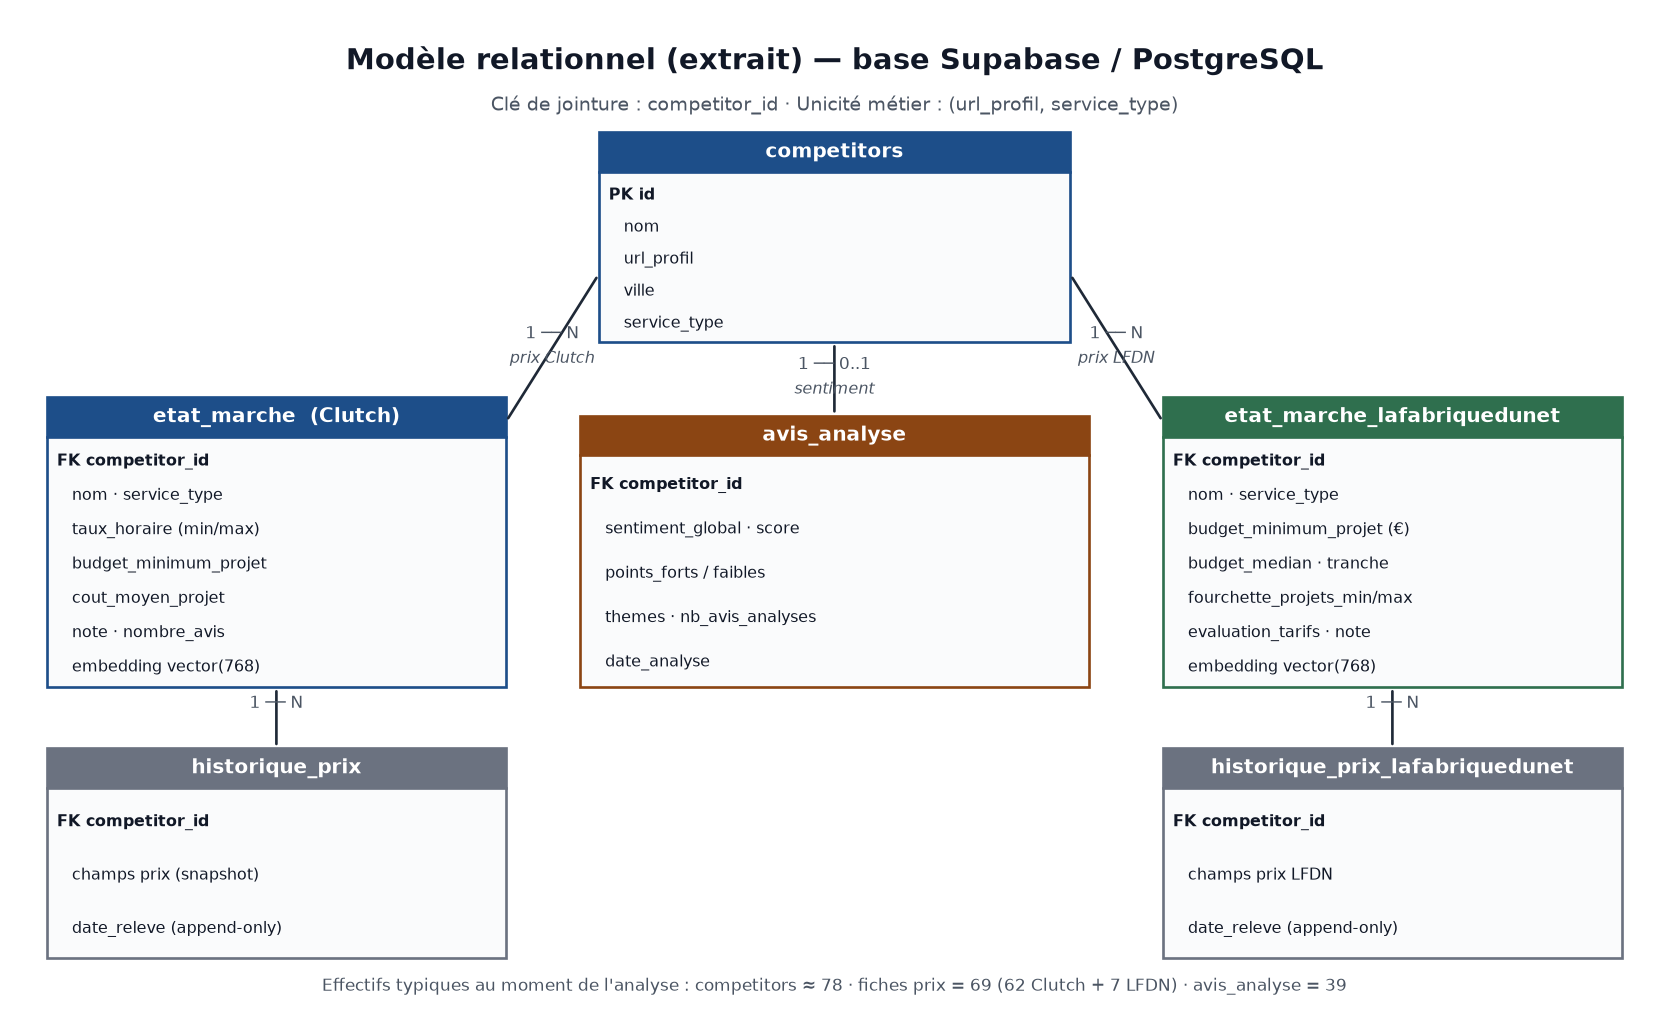
\includegraphics[width=0.95\textwidth]{img/modele_relationnel.png}
\caption{Modèle relationnel (extrait) de la base Supabase/PostgreSQL.
Tables principales~: \texttt{competitors}, \texttt{etat\_marche}, \texttt{etat\_marche\_lafabriquedunet}, \texttt{avis\_analyse}, \texttt{historique\_prix}.
Date du schéma~: 15/09/2026 (état de la base au moment de l'analyse).
Population représentée~: $78$ identités dans \texttt{competitors}~; $69$ fiches prix ($62$ Clutch + $7$ La Fabrique du Net)~; $39$ analyses d'avis.
Exclusion / non représenté sur le schéma simplifié~: tables annexes de monitoring non nécessaires à la lecture du RAG.}
\label{fig:modele_relationnel}
\end{figure}

\subsection{Analyse exploratoire des données (EDA)}

Sur les 78 entreprises identifiées (mobile et web confondus), 69 (88\,\%) disposent d'au moins une
donnée de prix exploitable. Parmi ces 69, 39 (56.5\,\%) disposent en outre d'une analyse de sentiment
fondée sur des avis clients en nombre suffisant. Cet écart de couverture entre identité, prix et
sentiment reflète le filtrage qualité décrit en section 10.1 : certaines entreprises ont été exclues à
une étape parce que leurs données étaient trop incomplètes pour être exploitées de façon fiable à cette
étape précise, sans être nécessairement exclues des étapes précédentes.

La distribution des taux horaires minimums (Clutch) fait apparaître une nette asymétrie vers le haut de
l'échelle plutôt qu'une répartition centrée (Figure~\ref{fig:distribution_taux_horaire}) : le mode se
situe dans la tranche 100--149 \$/h, qui concentre à elle seule 22 des 43 agences web (51\,\%) et 6 des 19
agences mobile (32\,\%). Les profils mobile et web diffèrent sensiblement sur ce point : le mobile est
proportionnellement plus représenté dans les tranches basses et moyennes (25--99 \$/h, 11 agences sur 19,
soit 58\,\%), tandis que le web bascule plus nettement vers le haut de la fourchette. Les positions
extrêmes restent rares dans les deux cas (une seule agence de chaque profil en dessous de 25 \$/h, et une
seule au-delà de 140 \$/h), ce qui situe l'essentiel du marché observé entre 25 et 150 \$/h. Les
statistiques descriptives complètes par \texttt{service\_type} (moyenne, médiane, écart-type) sont données
par \texttt{rapport\_eda.md}.

La répartition du sentiment global issu de l'extraction LLM montre une très forte prédominance des avis
positifs (37 entreprises, 95\,\%) sur les avis négatifs (2 entreprises, 5\,\%) ; aucun avis n'a été classé
neutre sur cet échantillon (voir Figure~\ref{fig:repartition_sentiment}).

Mise en regard de la note déclarée par les clients (sur 5), la corrélation entre la note globale et le
score de sentiment attribué par le LLM est de $r = 0.16$ ($n = 22$, $p = 0.47$). Ce calcul porte
volontairement sur le sous-ensemble d'entreprises pour lesquelles la note \emph{et} les avis analysés
proviennent de la même source de référence, Clutch ou La Fabrique du Net --- et non sur des avis
collectés ailleurs (réseaux sociaux, Google, etc.), afin de comparer deux mesures homogènes issues d'un
même corpus d'avis plutôt que deux corpus distincts. Sur ces 22 entreprises, le nombre d'avis analysés
(\texttt{nb\_avis\_analyses}) est d'ailleurs très proche du nombre d'avis brut relevé par la plateforme
(\texttt{nombre\_avis}) --- par exemple 36 avis Clutch pour 37 avis analysés chez Redlab Agency, ou 51
pour 53 chez SolveIt --- confirmant que l'analyse de sentiment porte bien, pour ce sous-groupe, sur le
même corpus d'avis que la note affichée.

Cette corrélation, faible et non significative au seuil usuel de 5\,\%, doit être interprétée avec
prudence : le sous-échantillon retenu présente une variance structurellement réduite (notes comprises
entre 4.18 et 5.0, scores de sentiment entre 0.88 et 1.00), ce qui limite mécaniquement l'amplitude
d'une corrélation linéaire mesurable. Il faut par ailleurs souligner que \texttt{note = 0} dans
\texttt{etat\_marche} signifie l'absence d'avis sur la plateforme source (Clutch ou La Fabrique du Net),
et non l'absence totale d'avis pour l'entreprise concernée : 17 entreprises supplémentaires disposent
d'avis analysés (\texttt{nb\_avis\_analyses} > 0) issus d'autres sources, sans note de référence
comparable associée à ce même corpus, et sont de ce fait exclues du calcul de corrélation ci-dessus ---
un biais de sélection méthodologiquement assumé plutôt qu'une simple donnée manquante aléatoire.

Les deux indicateurs peuvent ainsi refléter des dimensions différentes de l'expérience client : la note
traduit une évaluation globale et explicite, tandis que le score de sentiment repose sur l'analyse
sémantique du contenu textuel de l'avis. Compte tenu du faible nombre d'observations et de l'absence de
significativité statistique, ce résultat ne constitue pas une validation directe de la fiabilité de
l'extraction zero-shot ; il met plutôt en évidence la complémentarité potentielle entre l'évaluation
quantitative déclarée et l'analyse qualitative automatisée des avis, ainsi que l'intérêt de traiter les
deux sources de notation comme des populations distinctes plutôt que comme un seul échantillon homogène.

\subsection{Visualisations et interprétations statistiques}

Les figures suivantes, produites par \texttt{analyse\_donnees.py}, illustrent les principaux résultats présentés précédemment. Pour chaque figure sont indiqués~: la date d'extraction des données, la population étudiée, les règles d'exclusion, ainsi que les effectifs ($n$) en complément des pourcentages.

\begin{itemize}
\item \textbf{Figure~\ref{fig:couverture_donnees}} --- Couverture des données par étape du pipeline (identité $\rightarrow$ prix $\rightarrow$ sentiment).
\item \textbf{Figure~\ref{fig:distribution_taux_horaire}} --- Distribution des taux horaires Clutch par type de service.
\item \textbf{Figure~\ref{fig:distribution_notes_source}} --- Distribution des notes globales par source.
\item \textbf{Figure~\ref{fig:repartition_sentiment}} --- Répartition du sentiment global issu de l'analyse LLM.
\item \textbf{Figure~\ref{fig:correlation_note_sentiment}} --- Corrélation entre note déclarée et score de sentiment LLM.
\end{itemize}

\begin{figure}[H]
\centering
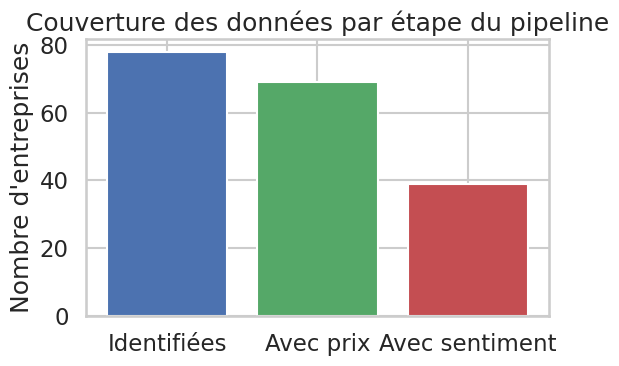
\includegraphics[width=0.8\textwidth]{img/couverture_donnees.png}
\caption{Couverture des données par étape du pipeline (identité, prix, sentiment).
Effectifs~: $78$ entreprises identifiées ($100\,\%$)~; $69$ avec prix exploitable ($88\,\%$)~; $39$ avec analyse de sentiment ($50\,\%$ des identifiées, $56{,}5\,\%$ des fiches prix).
Date d'extraction~: 15/09/2026.
Population~: ensemble des concurrents collectés (Clutch et La Fabrique du Net, profils web et mobile).
Exclusion~: $9$ entreprises sans donnée de prix exploitable ni avis utilisable (champs \textit{Undisclosed} / absence totale d'information).}
\label{fig:couverture_donnees}
\end{figure}

\begin{figure}[H]
\centering
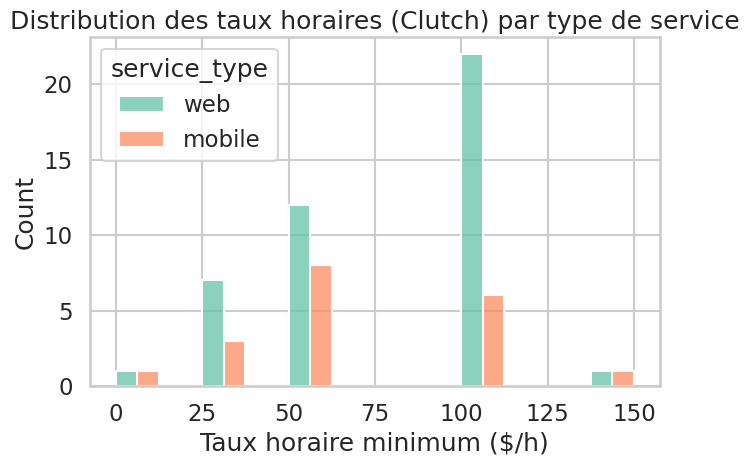
\includegraphics[width=0.8\textwidth]{img/distribution_taux_horaire.png}
\caption{Distribution des taux horaires Clutch par type de service (effectifs et pourcentages par tranche).
Mode~: tranche $100$--$149\,\$/\text{h}$ --- $22/43$ agences web ($51\,\%$) et $6/19$ agences mobile ($32\,\%$).
Date d'extraction~: 15/09/2026.
Population~: fiches Clutch avec taux horaire renseigné ($n_{\text{web}}=43$, $n_{\text{mobile}}=19$).
Exclusion~: entreprises La Fabrique du Net (pas de taux horaire)~; fiches Clutch sans taux horaire parseable~; valeurs \texttt{"No content available"} / \textit{Undisclosed}.}
\label{fig:distribution_taux_horaire}
\end{figure}

\begin{figure}[H]
\centering
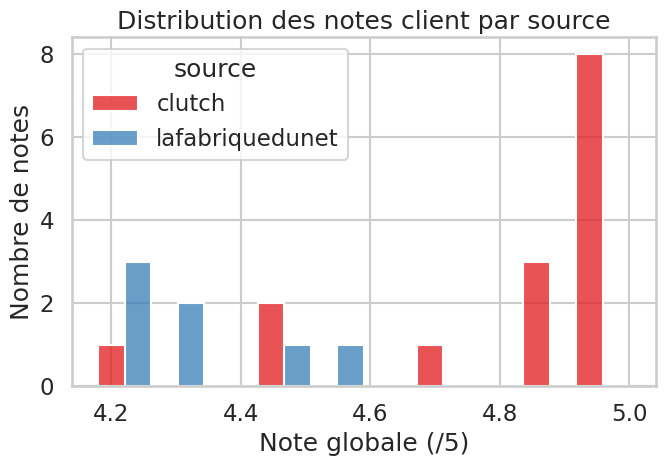
\includegraphics[width=0.8\textwidth]{img/distribution_notes_source.png}
\caption{Distribution des notes globales par source (effectifs $n$ et pourcentages par classe de note).
Date d'extraction~: 15/09/2026.
Population~: fiches dont la note source est renseignée et strictement positive (sous-ensemble de \texttt{etat\_marche} / \texttt{etat\_marche\_lafabriquedunet}).
Exclusion~: notes nulles ou absentes ($note = 0$ ou non renseignée), qui ne correspondent pas nécessairement à une absence d'avis hors source (cf.\ distinction avec \texttt{avis\_analyse}).}
\label{fig:distribution_notes_source}
\end{figure}

\begin{figure}[H]
\centering
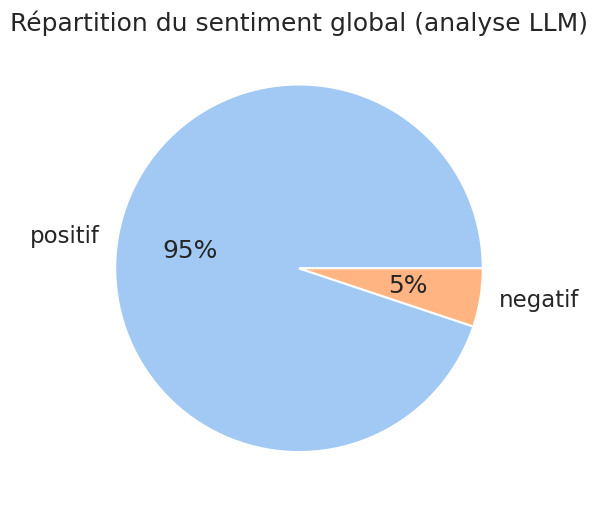
\includegraphics[width=0.8\textwidth]{img/repartition_sentiment.png}
\caption{Répartition du sentiment global issu de l'analyse LLM.
Effectifs~: positif $37$ ($95\,\%$)~; négatif $2$ ($5\,\%$)~; neutre $0$ ($0\,\%$)~; $n=39$.
Date d'extraction~: 15/09/2026 (date d'analyse des avis).
Population~: concurrents présents dans \texttt{avis\_analyse} ($n=39$).
Exclusion~: $30$ fiches prix sans analyse de sentiment (avis insuffisants ou non collectés).}
\label{fig:repartition_sentiment}
\end{figure}

\begin{figure}[H]
\centering
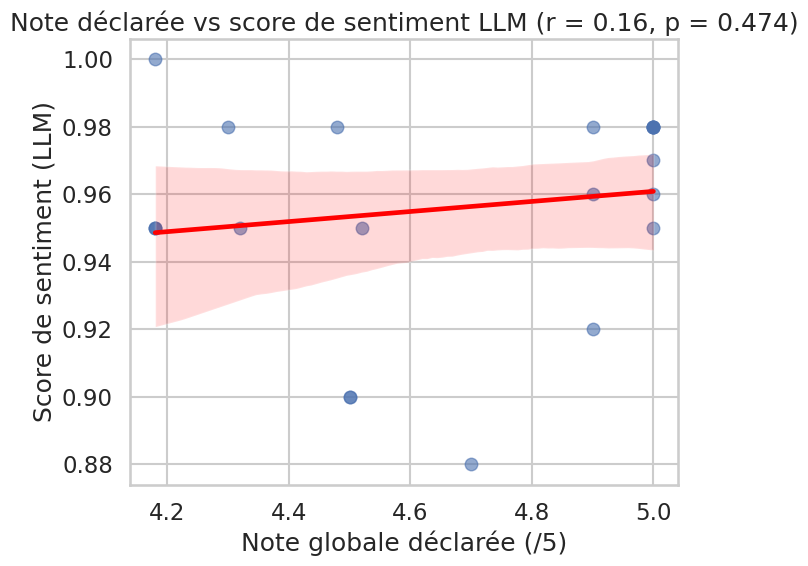
\includegraphics[width=0.8\textwidth]{img/correlation_note_sentiment.png}
\caption{Corrélation entre note déclarée et score de sentiment LLM ($r = 0{,}16$, $n = 22$, $p = 0{,}47$).
Date d'extraction~: 15/09/2026.
Population~: entreprises pour lesquelles la note \emph{et} les avis analysés proviennent de la même source (Clutch ou La Fabrique du Net), $n=22$.
Exclusion~: couples note/avis issus de sources hétérogènes~; entreprises sans note source ou sans score de sentiment.}
\label{fig:correlation_note_sentiment}
\end{figure}

\subsection{Réduction de dimension des embeddings (PCA, t-SNE)}

Les embeddings vectoriels calculés par le système de RAG (Gemini, 768 dimensions) constituent un objet
d'analyse naturel : ils sont censés capturer une notion de proximité sémantique entre profils de
concurrents, notion qui sous-tend directement la recherche par similarité cosinus utilisée en production
(section 4.2.3). Une projection en deux dimensions via PCA, puis via t-SNE, permet d'évaluer visuellement
si cette hypothèse se vérifie.

La PCA, projection linéaire, ne conserve que 21\,\% de la variance totale sur ses deux premières
composantes (Figure~\ref{fig:pca_embeddings}) --- un taux faible, mais attendu compte tenu de la
dimensionnalité élevée des embeddings (768D) : une projection 2D ne peut capturer qu'une fraction limitée
de la structure d'un espace de cette dimension, et ce chiffre doit être lu comme une limite de la
visualisation plutôt que comme une caractéristique des embeddings eux-mêmes.

Le nuage de points fait apparaître, visuellement, un clivage net en deux groupes selon l'axe principal de
la PCA. Avant d'attribuer cette séparation à une similarité sémantique entre profils d'agences --- ce qui
aurait constitué un argument de validation pour l'architecture RAG --- plusieurs facteurs de confusion ont
été systématiquement écartés par diagnostic croisé (coloration successive du nuage de points selon
différentes variables) : ni le \texttt{service\_type} (mobile vs web), ni la source de collecte (Clutch vs
La Fabrique du Net) ne permettent d'expliquer ce clivage, les deux catégories étant mélangées dans les
deux groupes.

En revanche, la présence ou l'absence d'avis clients (\texttt{note > 0} ou \texttt{nombre\_avis > 0})
explique la quasi-totalité du clivage observé (Figure~\ref{fig:pca_diagnostic_avis}) : les 22 entreprises
disposant d'avis clients se trouvent \emph{toutes} dans le groupe de droite, tandis que le groupe de
gauche est composé à 100\,\% (30/30) d'entreprises sans aucun avis. Le groupe de droite reste néanmoins
hétérogène, puisqu'il contient également 17 entreprises sans avis. Cette structure suggère que l'axe
principal de variance des embeddings reflète en grande partie la présence ou l'absence de contenu textuel
lié aux avis clients dans les champs utilisés pour construire la représentation vectorielle, plutôt qu'une
similarité intrinsèque de positionnement métier entre agences.

Le t-SNE, projection non linéaire optimisée pour préserver les voisinages locaux, fait apparaître une
structure plus fine que la PCA, avec en particulier un sous-groupe compact et isolé correspondant
exclusivement aux sept entreprises issues de La Fabrique du Net --- cohérent avec le fait que ces sept
entreprises disposent toutes d'avis clients (et se classent donc, comme attendu, dans le groupe "avec
avis" de droite en PCA), mais leur isolement encore plus marqué en t-SNE peut également refléter une
différence de langue du contenu source (profils rédigés en français pour La Fabrique du Net, en anglais
pour Clutch), un facteur de confusion supplémentaire qui n'a pas été formellement écarté ici et qui
constitue une limite à documenter.

Ce résultat doit donc être interprété comme un indice partiellement positif mais nuancé : les embeddings
capturent bien une structure exploitable en 2D, mais celle-ci est dominée --- pour son axe principal --- par
un artefact de complétude des données (présence/absence d'avis clients dans le texte source) plutôt que par
un signal de similarité purement métier entre concurrents comparables. Cette observation ne remet pas en
cause le fonctionnement du RAG en tant que tel, la similarité cosinus opérant en haute dimension (768D) où
d'autres axes de variance, non visibles sur cette projection 2D, peuvent porter un signal sémantique plus
pertinent ; elle invite cependant à la prudence dans l'interprétation purement visuelle de cette validation,
et suggère une piste d'amélioration future : exclure les champs liés aux avis de la construction de
l'embedding, ou les traiter séparément, afin d'isoler un signal de similarité de positionnement métier plus
directement exploitable pour la recherche de concurrents comparables.

\begin{figure}[H]
\centering
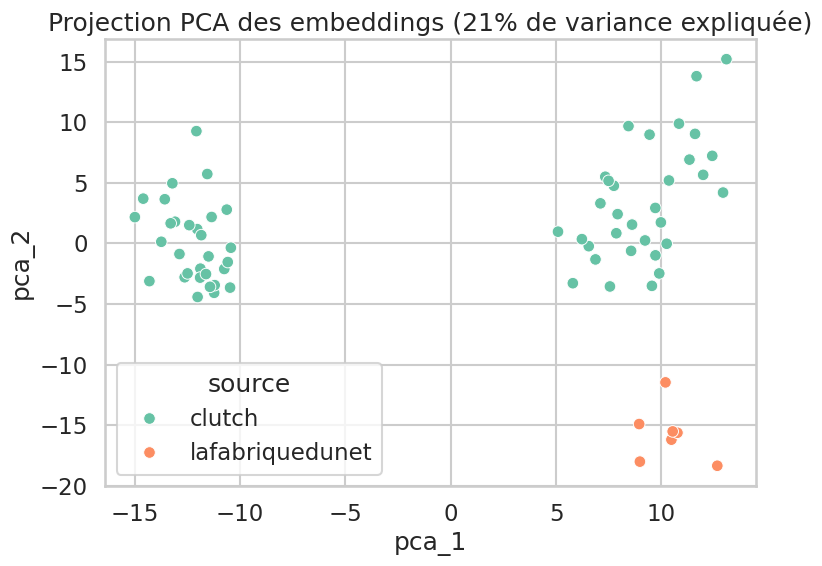
\includegraphics[width=0.8\textwidth]{img/pca_embeddings.png}
\caption{Projection PCA des embeddings, colorée par source ($21\,\%$ de variance expliquée sur les deux premières composantes~; $n=69$ fiches indexées).
Date d'extraction / indexation~: 15/09/2026.
Population~: embeddings Gemini (768 dimensions) des fiches présentes en base ($n=69$).
Exclusion~: concurrents sans embedding (aucun au moment de l'analyse)~; entreprises filtrées en amont ($78 \rightarrow 69$).}
\label{fig:pca_embeddings}
\end{figure}

\begin{figure}[H]
\centering
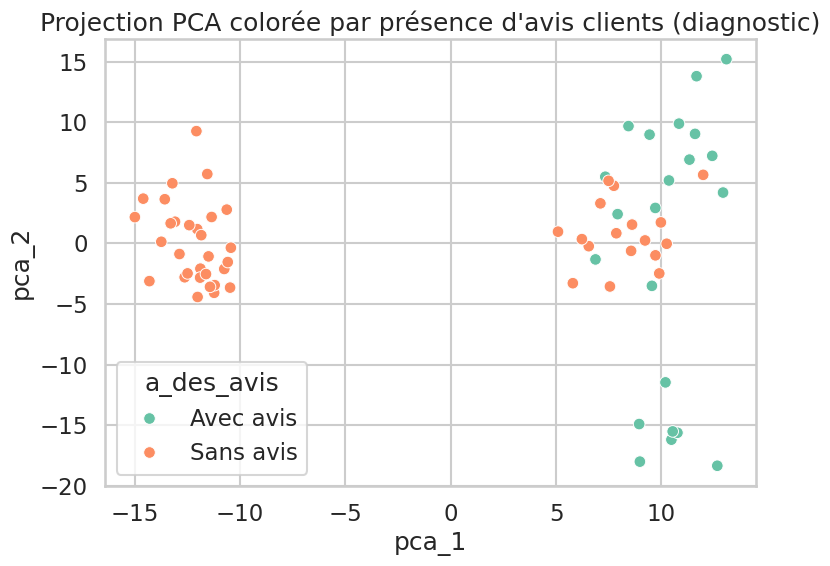
\includegraphics[width=0.8\textwidth]{img/pca_par_presence_avis.png}
\caption{Diagnostic PCA coloré par présence d'avis clients.
Effectifs~: groupe « avec avis » entièrement composé des $22$ entreprises ayant des avis source~; groupe « sans avis »~: $30/30$ ($100\,\%$) sans avis~; le groupe de droite reste hétérogène ($17$ sans avis également).
Date d'extraction / indexation~: 15/09/2026.
Population~: mêmes $n=69$ embeddings que la figure~\ref{fig:pca_embeddings}.
Exclusion~: idem~; coloration fondée sur $note > 0$ ou $nombre\_avis > 0$ dans les tables de prix.}
\label{fig:pca_diagnostic_avis}
\end{figure}

\begin{figure}[H]
\centering
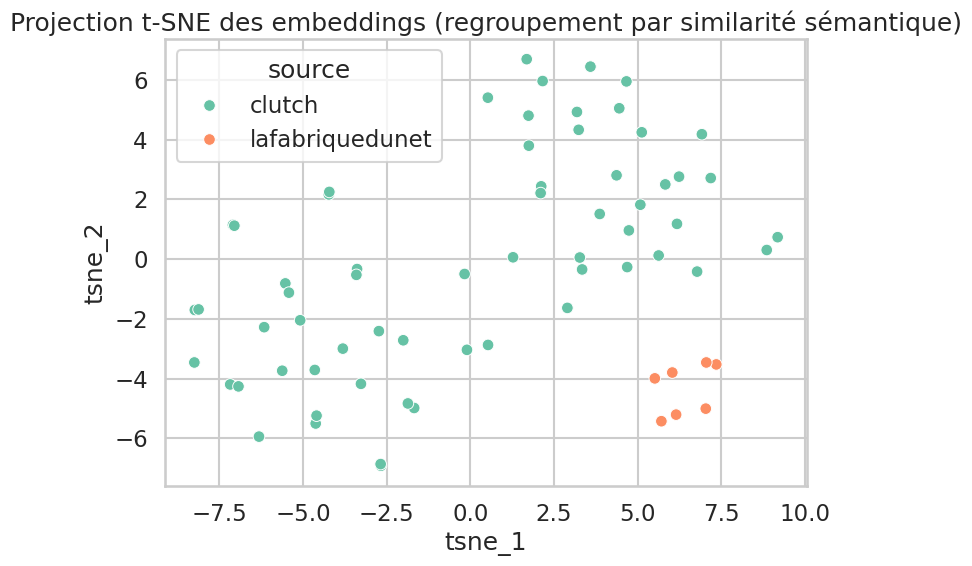
\includegraphics[width=0.8\textwidth]{img/tsne_embeddings.png}
\caption{Projection t-SNE des embeddings.
Sous-groupe isolé~: $7$ entreprises La Fabrique du Net ($100\,\%$ de cette source).
Date d'extraction / indexation~: 15/09/2026.
Population~: $n=69$ embeddings indexés.
Exclusion~: idem PCA~; interprétation prudente (artefact possible de langue FR vs EN du contenu source).}
\label{fig:tsne_embeddings}
\end{figure}